% Options for packages loaded elsewhere
\PassOptionsToPackage{unicode}{hyperref}
\PassOptionsToPackage{hyphens}{url}
%
\documentclass[
  openany]{book}
\usepackage{amsmath,amssymb}
\usepackage{lmodern}
\usepackage{ifxetex,ifluatex}
\ifnum 0\ifxetex 1\fi\ifluatex 1\fi=0 % if pdftex
  \usepackage[T1]{fontenc}
  \usepackage[utf8]{inputenc}
  \usepackage{textcomp} % provide euro and other symbols
\else % if luatex or xetex
  \usepackage{unicode-math}
  \defaultfontfeatures{Scale=MatchLowercase}
  \defaultfontfeatures[\rmfamily]{Ligatures=TeX,Scale=1}
\fi
% Use upquote if available, for straight quotes in verbatim environments
\IfFileExists{upquote.sty}{\usepackage{upquote}}{}
\IfFileExists{microtype.sty}{% use microtype if available
  \usepackage[]{microtype}
  \UseMicrotypeSet[protrusion]{basicmath} % disable protrusion for tt fonts
}{}
\makeatletter
\@ifundefined{KOMAClassName}{% if non-KOMA class
  \IfFileExists{parskip.sty}{%
    \usepackage{parskip}
  }{% else
    \setlength{\parindent}{0pt}
    \setlength{\parskip}{6pt plus 2pt minus 1pt}}
}{% if KOMA class
  \KOMAoptions{parskip=half}}
\makeatother
\usepackage{xcolor}
\IfFileExists{xurl.sty}{\usepackage{xurl}}{} % add URL line breaks if available
\IfFileExists{bookmark.sty}{\usepackage{bookmark}}{\usepackage{hyperref}}
\hypersetup{
  pdftitle={Documento Técnico N°6: Ciencia de Datos para el Turismo},
  pdfauthor={Dirección Nacional de Mercados y Estadísticas - Subsecretaría de Desarrollo Estratégico},
  hidelinks,
  pdfcreator={LaTeX via pandoc}}
\urlstyle{same} % disable monospaced font for URLs
\usepackage{longtable,booktabs,array}
\usepackage{calc} % for calculating minipage widths
% Correct order of tables after \paragraph or \subparagraph
\usepackage{etoolbox}
\makeatletter
\patchcmd\longtable{\par}{\if@noskipsec\mbox{}\fi\par}{}{}
\makeatother
% Allow footnotes in longtable head/foot
\IfFileExists{footnotehyper.sty}{\usepackage{footnotehyper}}{\usepackage{footnote}}
\makesavenoteenv{longtable}
\usepackage{graphicx}
\makeatletter
\def\maxwidth{\ifdim\Gin@nat@width>\linewidth\linewidth\else\Gin@nat@width\fi}
\def\maxheight{\ifdim\Gin@nat@height>\textheight\textheight\else\Gin@nat@height\fi}
\makeatother
% Scale images if necessary, so that they will not overflow the page
% margins by default, and it is still possible to overwrite the defaults
% using explicit options in \includegraphics[width, height, ...]{}
\setkeys{Gin}{width=\maxwidth,height=\maxheight,keepaspectratio}
% Set default figure placement to htbp
\makeatletter
\def\fps@figure{htbp}
\makeatother
\setlength{\emergencystretch}{3em} % prevent overfull lines
\providecommand{\tightlist}{%
  \setlength{\itemsep}{0pt}\setlength{\parskip}{0pt}}
\setcounter{secnumdepth}{5}
  %%% REFERENCIAS
        \usepackage{hyperref}
        % links del indice en negro; citas y URL en azul
        \hypersetup{colorlinks = true, urlcolor={blue}, 
        citecolor={blue}, linkcolor ={blue}}
\usepackage[spanish]{babel} % Idiomas en los que se escribe el documento. 
\usepackage{booktabs}
\usepackage{amsthm}

\usepackage[final]{pdfpages}

\makeatletter
\def\thm@space@setup{%
  \thm@preskip=8pt plus 2pt minus 4pt
  \thm@postskip=\thm@preskip
}
\makeatother
\let\oldmaketitle\maketitle
\AtBeginDocument{\let\maketitle\relax}
\ifluatex
  \usepackage{selnolig}  % disable illegal ligatures
\fi

\title{Documento Técnico N°6: Ciencia de Datos para el Turismo}
\usepackage{etoolbox}
\makeatletter
\providecommand{\subtitle}[1]{% add subtitle to \maketitle
  \apptocmd{\@title}{\par {\large #1 \par}}{}{}
}
\makeatother
\subtitle{El turismo desde la perspectiva de la oferta: actividad y empleo}
\author{Dirección Nacional de Mercados y Estadísticas - Subsecretaría de Desarrollo Estratégico}
\date{18 de August de 2021}

\begin{document}
\maketitle

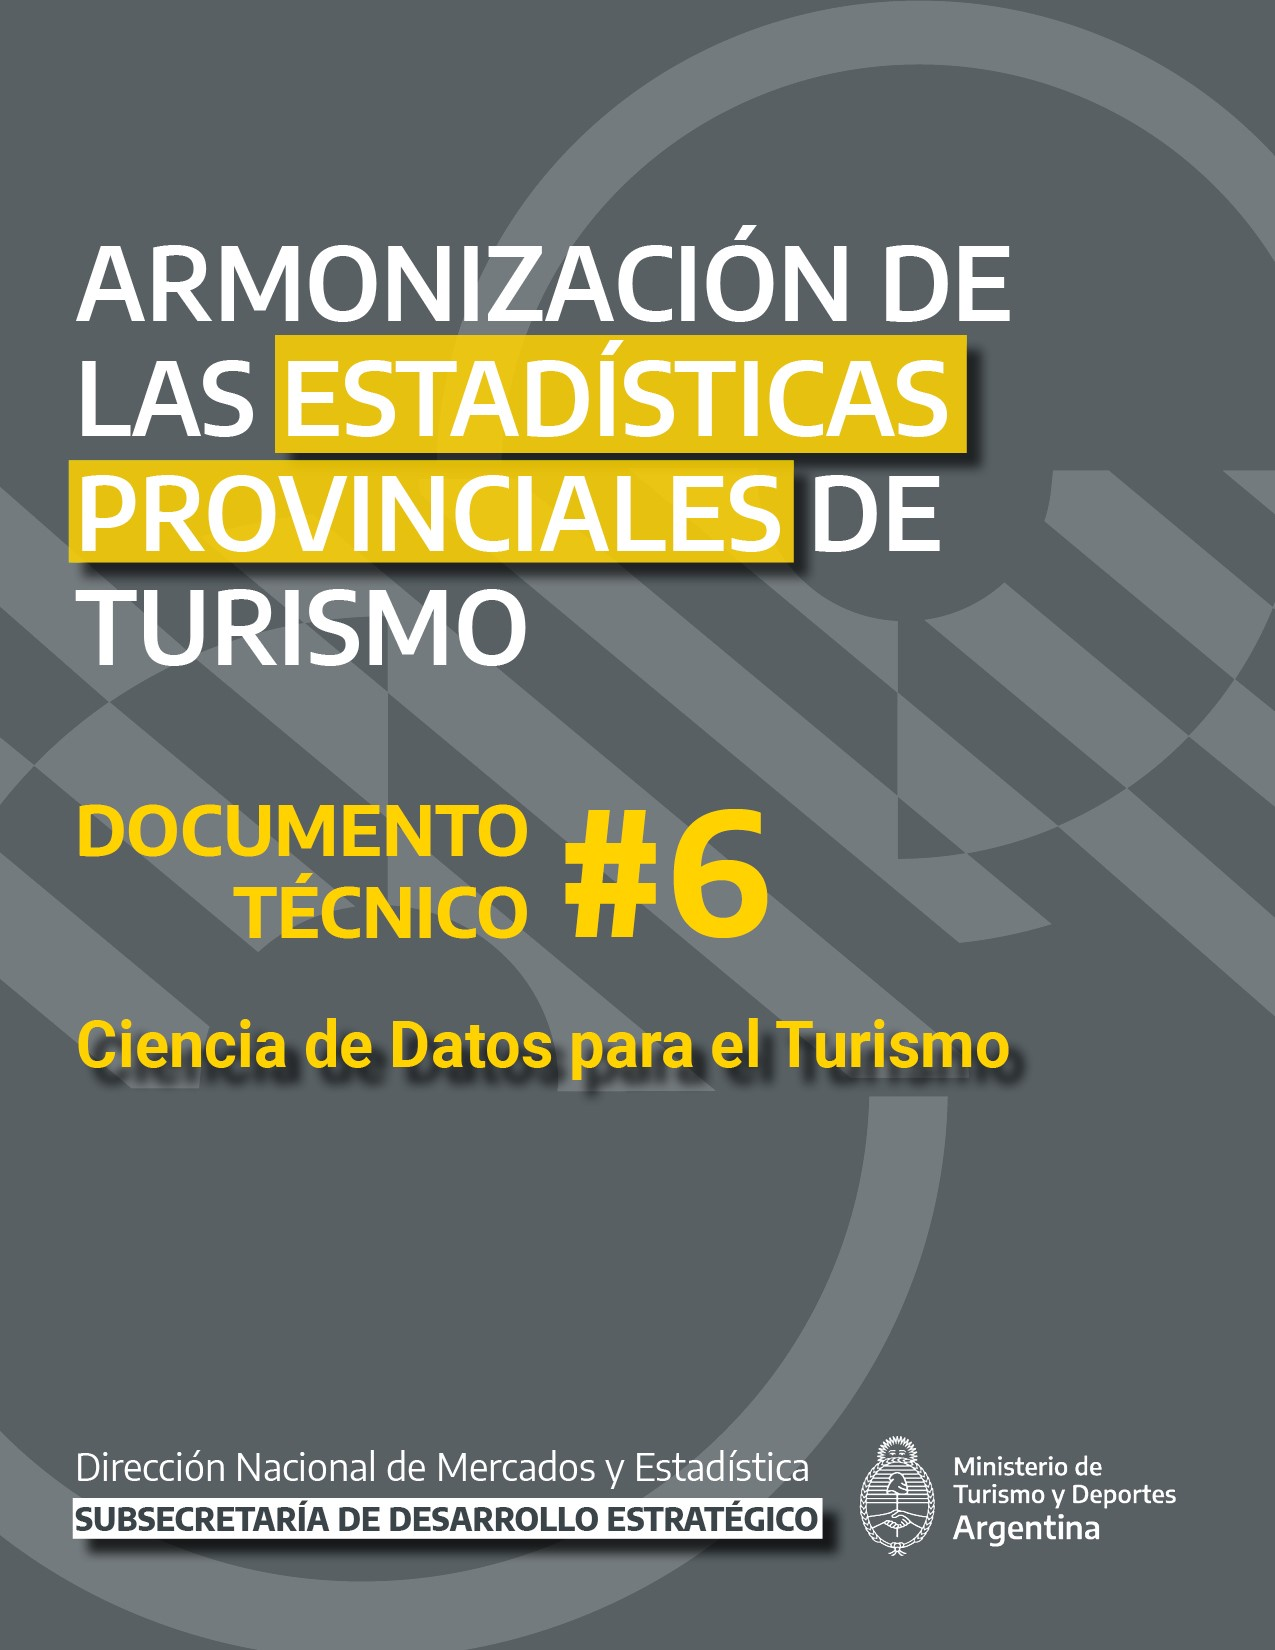
\includepdf[pages={1}, scale=1]{DT6Portada.pdf}
\newpage

\let\maketitle\oldmaketitle
\maketitle

{
\setcounter{tocdepth}{1}
\tableofcontents
}
\hypertarget{presentaciuxf3n}{%
\chapter*{Presentación}\label{presentaciuxf3n}}
\addcontentsline{toc}{chapter}{Presentación}

El presente documento, \textbf{Ciencia de Datos para Turismo}, se enmarca en el proyecto de Armonización de las Estadísticas de Turismo en las Provincias de la \href{https://www.yvera.tur.ar/estadistica/}{Dirección Nacional de Mercados y Estadística de la Subsecretaría de Desarrollo Estratégico del Ministerio de Turismo y Deportes}. El objetivo general de este proyecto es contribuir con propuestas metodológicas para los sistemas de estadísticas de turismo provinciales que orienten a producir indicadores provinciales básicos y comparables.

Además de este, se encuentra disponible una serie de documentos técnicos que abordan otras problemáticas vinculadas a la producción de estadística de turismo:

\begin{itemize}
\item
  \href{https://dnme-minturdep.github.io/DT1_medicion_turismo/}{Documento Técnico \#1}: Conceptos y elementos básicos para la medición provincial de los turistas
\item
  \href{https://dnme-minturdep.github.io/DT2_encuestas/}{Documento Técnico \#2}: Propuestas metodológicas para las encuestas de ocupación en alojamientos turísticos
\item
  \href{https://dnme-minturdep.github.io/DT3_registros_adminsitrativos/}{Documento Técnico \#3}: Descripción, análisis y utilización de los Registros Administrativos para la medición del Turismo
\item
  \href{https://dnme-minturdep.github.io/DT4_perfiles/}{Documento Técnico \#4}: Propuestas Metodológicas para las Encuestas de Perfil del Visitante
\item
  \href{https://dnme-minturdep.github.io/DT5_actividad_empleo/}{Documento Técnico \#5}: Medición de la contribución económica del turismo: actividad y empleo
\end{itemize}

\hypertarget{documento-tuxe9cnico-nuxba6---resumen}{%
\subsection*{Documento Técnico Nº6 - Resumen}\label{documento-tuxe9cnico-nuxba6---resumen}}
\addcontentsline{toc}{subsection}{Documento Técnico Nº6 - Resumen}

\end{document}
